\documentclass[10pt]{article}
% header.tex
% this is where you load pacakges, specify custom formats, etc.

\usepackage[left=1in,right=1in,top=1in,footskip=25pt]{geometry} 
% \usepackage{changepage}
\usepackage{amsmath,amsthm,amssymb,amsfonts}
\usepackage{mathtools}
\usepackage{bm}
\usepackage{bbm}
\usepackage{mathrsfs}
\usepackage{accents}
\usepackage{xspace}
% enumitem for custom lists
\usepackage{enumitem}
% Load dsfont this to get proper indicator function (bold 1) with \mathds{1}:
\usepackage{dsfont}
\usepackage{centernot}

\usepackage[ruled,vlined,linesnumbered]{algorithm2e}
\usepackage{multirow}
\usepackage{booktabs}
\makeatletter
% Booktab style
\renewcommand*{\@algocf@pre@ruled}{\hrule height\heavyrulewidth depth0pt \kern\belowrulesep}
\renewcommand*{\algocf@caption@ruled}{\box\algocf@capbox\kern\aboverulesep\hrule height\lightrulewidth\kern\belowrulesep}
\renewcommand*{\@algocf@post@ruled}{\kern\aboverulesep\hrule height\heavyrulewidth\relax}
\makeatother

\usepackage[usenames,dvipsnames]{xcolor}

% set up commenting code (I will use this during marking)
\definecolor{CommentColor}{rgb}{0,.50,.50}
\newcounter{margincounter}
\newcommand{\displaycounter}{{\arabic{margincounter}}}
\newcommand{\incdisplaycounter}{{\stepcounter{margincounter}\arabic{margincounter}}}
\newcommand{\COMMENT}[1]{\textcolor{CommentColor}{$\,^{(\incdisplaycounter)}$}\marginpar{\scriptsize\textcolor{CommentColor}{ {\tiny $(\displaycounter)$} #1}}}

\usepackage{appendix}

% set up graphics
\usepackage{graphicx}
\DeclareGraphicsExtensions{.pdf,.png,.jpg}
\graphicspath{{fig/}}
\usepackage{float}

\usepackage[sorting=nyt,backend=biber,bibstyle=apa,citestyle=apa,giveninits=true]{biblatex}
\setlength\bibitemsep{1.5\itemsep}

\usepackage{fancyhdr}
\pagestyle{fancy}
\setlength{\headheight}{40pt}

%%%%%%%%%%%%%%%%%%%%%%%%%%%%%%%%%%%%%%%%%%%%%%%%%%%%%%%%%%%%%%%%%%%%%%%%%%%%%%%%%%%%
% most other packages you might use should be loaded before hyperref
%%%%%%%%%%%%%%%%%%%%%%%%%%%%%%%%%%%%%%%%%%%%%%%%%%%%%%%%%%%%%%%%%%%%%%%%%%%%%%%%%%%%

% Set up hyperlinks:
\definecolor{RefColor}{rgb}{0,0,.65}
\usepackage[colorlinks,linkcolor=RefColor,citecolor=RefColor,urlcolor=RefColor]{hyperref}

\usepackage[capitalize]{cleveref}
\crefname{appsec}{Appendix}{Appendices} % you can tell cleveref what to call things

\renewenvironment{abstract}
 {\par\noindent\textbf{\abstractname.}\ \ignorespaces}
 {\par\medskip}
% defs.tex
% this is where you define custom notation, commands, etc.


%%
% full alphabets of different styles
%%

% bf series
\def\bfA{\mathbf{A}}
\def\bfB{\mathbf{B}}
\def\bfC{\mathbf{C}}
\def\bfD{\mathbf{D}}
\def\bfE{\mathbf{E}}
\def\bfF{\mathbf{F}}
\def\bfG{\mathbf{G}}
\def\bfH{\mathbf{H}}
\def\bfI{\mathbf{I}}
\def\bfJ{\mathbf{J}}
\def\bfK{\mathbf{K}}
\def\bfL{\mathbf{L}}
\def\bfM{\mathbf{M}}
\def\bfN{\mathbf{N}}
\def\bfO{\mathbf{O}}
\def\bfP{\mathbf{P}}
\def\bfQ{\mathbf{Q}}
\def\bfR{\mathbf{R}}
\def\bfS{\mathbf{S}}
\def\bfT{\mathbf{T}}
\def\bfU{\mathbf{U}}
\def\bfV{\mathbf{V}}
\def\bfW{\mathbf{W}}
\def\bfX{\mathbf{X}}
\def\bfY{\mathbf{Y}}
\def\bfZ{\mathbf{Z}}

\def\bfb{\mathbf{b}}
\def\bfe{\mathbf{e}}
\def\bft{\mathbf{t}}
\def\bfy{\mathbf{y}}

\def\bfom{\bm{\omega}}
\def\bfOm{\bm{\Omega}}

% bb series
\def\bbA{\mathbb{A}}
\def\bbB{\mathbb{B}}
\def\bbC{\mathbb{C}}
\def\bbD{\mathbb{D}}
\def\bbE{\mathbb{E}}
\def\bbF{\mathbb{F}}
\def\bbG{\mathbb{G}}
\def\bbH{\mathbb{H}}
\def\bbI{\mathbb{I}}
\def\bbJ{\mathbb{J}}
\def\bbK{\mathbb{K}}
\def\bbL{\mathbb{L}}
\def\bbM{\mathbb{M}}
\def\bbN{\mathbb{N}}
\def\bbO{\mathbb{O}}
\def\bbP{\mathbb{P}}
\def\bbQ{\mathbb{Q}}
\def\bbR{\mathbb{R}}
\def\bbS{\mathbb{S}}
\def\bbT{\mathbb{T}}
\def\bbU{\mathbb{U}}
\def\bbV{\mathbb{V}}
\def\bbW{\mathbb{W}}
\def\bbX{\mathbb{X}}
\def\bbY{\mathbb{Y}}
\def\bbZ{\mathbb{Z}}

% cal series
\def\calA{\mathcal{A}}
\def\calB{\mathcal{B}}
\def\calC{\mathcal{C}}
\def\calD{\mathcal{D}}
\def\calE{\mathcal{E}}
\def\calF{\mathcal{F}}
\def\calG{\mathcal{G}}
\def\calH{\mathcal{H}}
\def\calI{\mathcal{I}}
\def\calJ{\mathcal{J}}
\def\calK{\mathcal{K}}
\def\calL{\mathcal{L}}
\def\calM{\mathcal{M}}
\def\calN{\mathcal{N}}
\def\calO{\mathcal{O}}
\def\calP{\mathcal{P}}
\def\calQ{\mathcal{Q}}
\def\calR{\mathcal{R}}
\def\calS{\mathcal{S}}
\def\calT{\mathcal{T}}
\def\calU{\mathcal{U}}
\def\calV{\mathcal{V}}
\def\calW{\mathcal{W}}
\def\calX{\mathcal{X}}
\def\calY{\mathcal{Y}}
\def\calZ{\mathcal{Z}}

\def\tildeU{\widetilde{U}}
\def\hatb{\widehat{\bfb}}
\def\hatOm{\widehat{\bfOm}}
\def\hatW{\widehat{\bfW}}
\def\hatmu{\widehat{\mu}}


%%%%%%%%%%%%%%%%%%%%%%%%%%%%%%%%%%%%%%%%%%%%%%%%%%%%%%%%%%
% text short-cuts
\def\iid{i.i.d.\ } %i.i.d.
\def\ie{i.e.\ }
\def\eg{e.g.\ }
\def\Polya{P\'{o}lya\ }
%%%%%%%%%%%%%%%%%%%%%%%%%%%%%%%%%%%%%%%%%%%%%%%%%%%%%%%%%%

%%%%%%%%%%%%%%%%%%%%%%%%%%%%%%%%%%%%%%%%%%%%%%%%%%%%%%%%%%
% quasi-universal probabilistic and mathematical notation
% my preferences (modulo publication conventions, and clashes like random vectors):
%   vectors: bold, lowercase
%   matrices: bold, uppercase
%   operators: blackboard (e.g., \mathbb{E}), uppercase
%   sets, spaces: calligraphic, uppercase
%   random variables: normal font, uppercase
%   deterministic quantities: normal font, lowercase
%%%%%%%%%%%%%%%%%%%%%%%%%%%%%%%%%%%%%%%%%%%%%%%%%%%%%%%%%%

% operators
\def\P{\bbP} %fundamental probability
\def\E{\bbE} %expectation
% conditional expectation
\DeclarePairedDelimiterX\bigCond[2]{[}{]}{#1 \;\delimsize\vert\; #2}
\newcommand{\conditional}[3][]{\bbE_{#1}\bigCond*{#2}{#3}}
\def\Law{\mathcal{L}} %law; this is by convention in the literature
\def\indicator{\mathds{1}} % indicator function

% sets and groups
\def\borel{\calB} %Borel sets
\def\sigAlg{\calA} %sigma-algebra
\def\filtration{\calF} %filtration
\def\grp{\calG} %group

% binary relations
\def\condind{{\perp\!\!\!\perp}} %independence/conditional independence
\def\equdist{\stackrel{\text{\rm\tiny d}}{=}} %equal in distribution
\def\equas{\stackrel{\text{\rm\tiny a.s.}}{=}} %euqal amost surely
\def\simiid{\sim_{\mbox{\tiny iid}}} %sampled i.i.d

% common vectors and matrices
\def\onevec{\mathbf{1}}
\def\iden{\mathbf{I}} % identity matrix
\def\supp{\text{\rm supp}}

% misc
% floor and ceiling
\DeclarePairedDelimiter{\ceilpair}{\lceil}{\rceil}
\DeclarePairedDelimiter{\floor}{\lfloor}{\rfloor}
\newcommand{\argdot}{{\,\vcenter{\hbox{\tiny$\bullet$}}\,}} %generic argument dot

\DeclareMathOperator*{\argmax}{arg\,max}
\DeclareMathOperator*{\argmin}{arg\,min}
%%%%%%%%%%%%%%%%%%%%%%%%%%%%%%%%%%%%%%%%%%%%%%%%%%%%%%%%%%

%%%%%%%%%%%%%%%%%%%%%%%%%%%%%%%%%%%%%%%%%%%%%%%%%%%%%%%%%%
%% some distributions
% continuous
\def\UnifDist{\text{\rm Unif}}
\def\BetaDist{\text{\rm Beta}}
\def\ExpDist{\text{\rm Exp}}
\def\GammaDist{\text{\rm Gamma}}
% \def\GenGammaDist{\text{\rm GGa}} %Generalized Gamma

% discrete
\def\BernDist{\text{\rm Bernoulli}}
\def\BinomDist{\text{\rm Binomial}}
\def\PoissonPlus{\text{\rm Poisson}_{+}}
\def\PoissonDist{\text{\rm Poisson}}
\def\NBPlus{\text{\rm NB}_{+}}
\def\NBDist{\text{\rm NB}}
\def\GeomDist{\text{\rm Geom}}
% \def\CRP{\text{\rm CRP}}
% \def\EGP{\text{\rm EGP}}
% \def\MittagLeffler{\text{\rm ML}}
%%%%%%%%%%%%%%%%%%%%%%%%%%%%%%%%%%%%%%%%%%%%%%%%%%%%%%%%%%

%%%%%%%%%%%%%%%%%%%%%%%%%%%%%%%%%%%%%%%%%%%%%%%%%%%%%%%%%%
% Project-specific notation should go here
% (Because it's at the end of the file, it can overwrite anything that came before.)

%e.g.,
\def\Laplacian{\calL}
%\def\P{\calP}

% combinatorial objects
\def\perm{\sigma} %fixed permutation
\def\Perm{\Sigma} %random permutation
\def\part{\pi} %fixed partition
\def\Part{\Pi} %random partition

% Kernels
\def\MMD{\mathrm{MMD}}
\def\hatMMD{\widehat{\MMD}}
\def\dhatMMD{\widehat{\vphantom{\rule{1.5pt}{5.5pt}}\smash{\hatMMD}}}
\def\d{\mathrm{d}}

\def\xo{x^{(1)}}
\def\xt{x^{(2)}}
\def\yo{y^{(1)}}
\def\yt{y^{(2)}}
\def\go{g^{(1)}}
\def\gtw{g^{(2)}}

% Theorems
\newtheorem{theorem}{Theorem}[section]
\newtheorem{proposition}[theorem]{Proposition}
\newtheorem{corollary}[theorem]{Corollary}
\renewcommand{\thetheorem}{\arabic{theorem}}


\newcommand{\mre}{\textsc{MRE}\xspace}
\newcommand{\Var}{\mathrm{Var}}
\newcommand{\bias}{\mathrm{bias}}
\newcommand{\barY}{\bar{Y}}

\newcommand{\T}{\top}

\newcommand\sbullet[1][.5]{\mathbin{\vcenter{\hbox{\scalebox{.75}{$\bullet$}}}}}

%%%%%%%%%%%%%%%%%%%%%%%%%%%%%%%%%%%%%%%%%%%%%%%%%%%%%%%%%%

\newcommand{\todo}{{\color{red}{TODO}}}

\title{Stepped Wedge Cluster Randomized Trials\\\vspace{0.5em}\large{STAT 548 Qualifying Paper}}
\author{Kenny Chiu}
\date{\today}

\bibliography{refs.bib}

\begin{document}

\maketitle

\vspace{2em}

\begin{abstract}
The work of \textcite{Hussey:2007} can be viewed as an entry-point to the study of stepped wedge cluster randomized trials. We summarize and comment on their work and address the shortcomings of their paper, which include missing technical details, a simulation study with a vague procedure, and a limited discussion of how their approach may be extended to more complicated trial contexts. We also highlight how their work has guided modern developments in the related literature. Our attempt at replicating their simulation study led to similar findings though we were seemingly unable to replicate their exact results.
\end{abstract}

\vspace{2em}


\section{Introduction}

The work of \textcite{Hussey:2007} can be viewed as an entry-point to the study of stepped wedge cluster randomized trials (SW-CRT), which is a type of experimental design that is particularly pragmatic compared to alternative designs that may also be used in similar contexts. In this report, we review the paper by \citeauthor{Hussey:2007}. We summarize the main ideas while filling in missing details, attempt to replicate and clarify their simulation study, and provide a critique of the paper. We also discuss how the literature on SW-CRTs has developed since the paper was published and highlight some of the common extensions to the basic model presented in the paper.
\\

This report is organized as follows: Section~\ref{sec:summary} summarizes the paper and provides additional details where we feel was missed in the original work; Section~\ref{sec:critique} discusses our perspective and commentary of the paper; Section~\ref{sec:simulation} describes our findings from our attempt to replicate the simulation study; Section~\ref{sec:extension} presents common modern extensions to the standard SW-CRT model; and Section~\ref{sec:discussion} concludes this report by summarizing our discussion. Appendix~\ref{apx} includes our longer technical explanations and derivations deferred from Section~\ref{sec:summary}. Appendix~\ref{apx:dataset} shows visualizations of example datasets generated through our simulation procedure described in Section~\ref{sec:simulation}.


\section{Summary and additional details} \label{sec:summary}

In this section, we summarize the main ideas of the paper by \textcite{Hussey:2007} and provide additional details where we feel are absent in the original paper. Our longer technical explanations and derivations are included in Appendix~\ref{apx} to avoid disrupting the flow of the summary.

\subsection{Context and motivation}

Cluster randomized trials (CRT) are characterized by the randomization to treatments being done at the group or cluster-level rather than at the individual-level, and it is typically assumed that the individuals within a cluster are correlated. CRTs are considered when it is inconvenient or not appropriate to administer an intervention to single individuals. \textcite{Hussey:2007} comment that the majority of CRT designs studied and employed (at the time of the paper) featured parallel designs where approximately half of the clusters are simultaneously given one intervention and the other half are simultaneously given another. While these parallel CRTs are convenient analytically, they may present problems in practice if, for example, there are logistical constraints that make delivering the intervention simultaneously across multiple clusters difficult. Other potential issues of parallel designs include ethical concerns where if there is an expectation that a new intervention improves on an existing one, then it may not be possible to withhold the new intervention from certain clusters.
\\

Our understanding is that the main objective of \citeauthor{Hussey:2007}' work is to promote the stepped wedge CRT design as an alternative solution that addresses the potential issues of the parallel design, and to provide an overview of how the data collected from such a design are analyzed. In addition, \citeauthor{Hussey:2007} also discuss certain statistical considerations of SW-CRT designs such as power and efficiency of estimators, and how these properties are affected by model assumptions and design parameters.

\subsection{SW-CRT design}

The SW-CRT design is a type of crossover design. However, unlike in standard crossover CRTs where clusters start with potentially different treatments and switch treatments at a determined time point, SW-CRT are characterized by
\begin{enumerate}

\item
the crossover being unidirectional where all clusters start with the same treatment (the control or an existing treatment) and end with the same treatment (the intervention), and

\item
the staggered times at which each cluster switches to the intervention (with the times being randomized across clusters).

\end{enumerate}
Figure~\ref{fig:designs} (taken from the original paper) clearly illustrates the differences between the discussed CRT designs.

\begin{figure}[H]
\centering
\begin{tabular}{@{}rr|c@{}}
\multicolumn{2}{l|}{\multirow{2}{*}{\textbf{Parallel}}} & \multicolumn{1}{r}{Time} \\
& & 1 \\
\hline
\multirow{4}{*}{Cluster} & 1 & 1 \\
& 2 & 1 \\
& 3 & 0 \\
& 4 & 0
\end{tabular}
\qquad
\begin{tabular}{@{}rr|cc@{}}
\multicolumn{2}{l|}{\multirow{2}{*}{\textbf{Crossover}}} & \multicolumn{2}{r}{Time} \\
& & 1 & 2 \\
\hline
\multirow{4}{*}{Cluster} & 1 & 1 & 0 \\
& 2 & 1 & 0 \\
& 3 & 0 & 1\\
& 4 & 0 & 1
\end{tabular}
\qquad
\begin{tabular}{@{}rr|ccccc@{}}
\multicolumn{2}{l|}{\textbf{Stepped}} & \multicolumn{5}{r}{Time} \\
 \multicolumn{2}{l|}{\textbf{wedge}} & 1 & 2 & 3 & 4 & 5 \\
\hline
\multirow{4}{*}{Cluster} & 1 & 0 & 1 & 1 & 1 & 1 \\
& 2 & 0 & 0 & 1 & 1 & 1 \\
& 3 & 0 & 0 & 0 & 1 & 1 \\
& 4 & 0 & 0 & 0 & 0 & 1
\end{tabular}
\caption{Example treatment schedules for parallel, crossover, and stepped wedge CRT designs. The control/existing treatment and the intervention are denoted 0 and 1, respectively. Figure slightly modified from \parencite{Hussey:2007}.}
\label{fig:designs}
\end{figure}

From Figure~\ref{fig:designs}, it can be seen how the SW-CRT design addresses the practical issues of the parallel design. Rather than simultaneously delivering the intervention to multiple groups, SW-CRTs stagger the delivery to clusters across different times, potentially alleviating logistical concerns. Furthermore, all clusters eventually receive the intervention, which avoids the problem of withholding the intervention from certain clusters. The SW-CRT design is not without its own complications, however. Staggering the times means that the duration of the study is elongated relative to the parallel and crossover designs. The unidirectional crossover also implies that time may be correlated with the effect of the intervention, which may lead to issues in estimation of the intervention effect when analyzing the data.
\\

Beyond the general characteristics of SW-CRTs described above, other considerations and design parameters (e.g., cluster sizes, number of clusters crossing over at each time point, new individuals in a cluster across time, etc.) will depend on the context of the specific study. \citeauthor{Hussey:2007} examine in detail the model for a SW-CRT under a specific setting. How the model changes to varying trial contexts are only briefly mentioned or, in the case of some variations, not discussed at all. We return to this point in our critique of the paper in Section~\ref{sec:critique} and again when we discuss model extensions in Section~\ref{sec:extension}.

\subsection{Assumed setting and SW-CRT model}

The SW-CRT model that \textcite{Hussey:2007} examine in their paper can be considered the ``basic'' or ``standard'' model and is based on a particular trial example.

\subsubsection{Expedited Partner Treatment trial}

The primary SW-CRT setting that \citeauthor{Hussey:2007} work under is based on the context of the \textit{Washington State Community Expedited Partner Treatment (EPT) Trial} that started in 2007 and ended in 2011 \parencite{Golden:2015}. The hypothesis of interest in this study was whether a public health program that increases the use of EPT decreases the prevalence of chlamydia in young women and the incidence of gonorrhea in WA state. The intervention---promotion of EPT and targeted provision of partner services---was instituted in 23 WA state local health jurisdictions (LHJ) across four waves separated by 6--9 months. Each wave included approximately six LHJs, and the order in which LHJs initiated the intervention were randomly assigned. The measured primary outcomes in the study included the prevalence of chlamydia in women aged 15--25 who tested positive in participating clinics and the incidence of gonorrhea in women as ascertained through public health reporting. Note that these outcomes are both treated as continuous.
\\

A key design aspect to consider for modeling is how the clusters and the individuals are defined. For example, in the chlamydia study of the EPT trial, each LHJ is treated as a cluster, and the women who were tested in a participating clinic during a particular timeframe are the individuals in the cluster. It is important to note that the women within a single cluster differ at different time points over the trial (i.e., the study features a cross-sectional SW-CRT). While the number of women who were tested varied between LHJs and across time within a single LHJ, there were likely more than enough women tested that only a sample of women for each time point and for each LHJ were sufficient for fitting a reasonable model. In such a scenario, it is analytically more convenient to take samples of equal sizes across LHJs and across time. \textcite{Hussey:2007} comment that for the gonorrhea study, because the incidence rates are much lower, taking samples of equal sizes across LHS and time may not be possible.
\\

Thus, motivated by the EPT trial, \citeauthor{Hussey:2007} examine the properties of a basic model for a continuous outcome, cross-sectional SW-CRT. Their discussion of the model is primarily under the assumption of equal cluster sizes, though they also examine the case of unequal sizes in their simulation study.

\subsubsection{SW-CRT model} \label{sec:model}

A linear mixed effects model (LMM) can be used to model the SW-CRT design described under the setting in the previous section. Assuming that there are $I$ clusters, $T$ time points, and $N$ individuals in each cluster at each time point, the mean for cluster $i$ at time $j$ can be defined as
\[
\mu_{ij} = \mu + \alpha_i + \beta_j + X_{ij}\theta
\]
where
\begin{itemize}

\item
$\mu$ is the overall mean across clusters and time,

\item
$\alpha_i\sim N(0,\tau^2)$ is a random effect for cluster $i\in\{1,\ldots,I\}$,

\item
$\beta_j$ is a fixed effect for time point $j\in\{1,\ldots,T-1\}$ (assuming $\beta_T=0$ for identifiability),

\item
$X_{ij}$ is a treatment indicator for cluster $i$ at time $j$ with 1 denoting that the cluster is in the intervention phase, and

\item
$\theta$ is the treatment effect of interest.

\end{itemize}
Using a slightly different notation from \citeauthor{Hussey:2007}, a model at the individual-level is then given by
\[
Y_{ijk} = \mu_{ij} + e_{ijk}
\]
where $e_{ijk}\sim N(0,\sigma^2)$ are i.i.d. noise, and this leads to a model at the cluster-level given by
\[
\barY_{ij} = \mu_{ij} + \frac{1}{N}\sum_{k=1}^Ne_{ijk} \;.
\]
As mentioned, this model can be considered the standard model for a SW-CRT design as the assumptions it makes are fairly basic. The model can be extended many ways depending on the setting of the specific study. We revisit this point in Section~\ref{sec:extension}.
\\

It is worth noting that two quantities obtainable from the model are also commonly referred to in the CRT literature. The intraclass correlation (ICC) $\rho=\frac{\tau^2}{\tau^2+\sigma^2}$ (and its induced variation inflation factor $1+(N-1)\rho$) and the coefficient of variation (CV) $\frac{\tau}{\mu}$ characterize the effect of the within-cluster correlation on the cluster mean variance and are often the parameters being adjusted in CRT simulation studies. We provide some intuition for these quantities in Appendix~\ref{apx:correlation}.


\subsection{Methods and analysis}

\textcite{Hussey:2007} discuss several ideas related to estimation and analysis of the simple model for a SW-CRT. We highlight the key points in this section. \citeauthor{Hussey:2007} mostly skip over technical explanations and derivations when discussing estimators and their statistical properties. We try to address these gaps in this section and in Appendix~\ref{apx}.

\subsubsection{Estimation of the treatment effect}

The general objective when analyzing data from a SW-CRT is to estimate and test the treatment effect $\theta$. When the variance components $\tau^2$ and $\sigma^2$ are known or if the clusters are approximately equal-sized, a cluster-level estimation of $\theta$ is possible using weighted least squares (WLS) to fit the cluster-level model described in Section~\ref{sec:model}. While this approach is useful for conducting a pre-trial power analysis, $\tau^2$ and $\sigma^2$ are generally unknown in practice. When the variance components are unknown and the clusters vary greatly in size, the WLS approach becomes less useful as the weights depend on the correct variances. In this case, an individual-level analysis using generalized linear mixed effects models (GLMM) or generalized estimating equations (GEE) would be the preferred approach. If there is a possibility of misspecifying the covariance structure, GEE would be preferred over GLMM as its parameter estimates remain consistent as long as the mean is correctly specified \parencite{Diggle:2002}. \textcite{Hussey:2007} caution that the LMM, GLMM, and GEE approaches all rely on asymptotic results, and so an analysis of a SW-CRT involving few clusters or time points may produce misleading findings.
\\

\citeauthor{Hussey:2007} remark that when there are no time effects on the outcome (i.e., when $\beta_j=0$ for all~$j$), estimation of the treatment effect $\theta$ can be done using a within-cluster analysis (an analysis based on comparing the control and intervention time periods for each cluster). This case also allows using a paired $t$-test to test the treatment effect where the two paired groups correspond to the control and the intervention time periods. However, the estimator for $\theta$ will be biased if the assumption that the time effects are trivial does not hold. We provide additional details about the estimator and the bias in Appendix~\ref{apx:estimator}.
\\

\citeauthor{Hussey:2007} also discuss the relative efficiency of the WLS estimator of the treatment effect compared to the within-cluster estimator. When there are no time effects, the WLS estimator is always more efficient than the within-cluster estimator unless if $\tau^2=0$. When there are time effects, the within-cluster estimator is more efficient (but likely biased). Note that there is an error in the efficiency given by \textcite{Hussey:2007} as pointed out by \textcite{Liao:2015}, though the above statements still hold. We also find that the proof by \textcite{Liao:2015}---which shows the greater efficiency of the WLS estimator compared to the within-cluster estimator---appears to hold even when $\tau^2=0$ in the case of no time effects. We provide further details for the efficiency and the proof for the no time effect-case in Appendix~\ref{apx:efficiency}.

\subsubsection{Power and relevant factors}

To approximate the power for testing the treatment effect against a simpler alternative $H_a: \theta=\theta_a$, \textcite{Hussey:2007} prescribe using a Wald test. The power for a two-tailed test of size $\alpha$ is approximately
\[
\text{power} \approx \Phi\left(\frac{\theta_a}{\sqrt{\Var(\hat{\theta})}} - Z_{1-\frac{\alpha}{2}}\right)
\]
where $\Phi$ is the cumulative distribution function of the standard normal and $Z_{1-\frac{\alpha}{2}}$ is the $\left(1-\frac{\alpha}{2}\right)$-th quantile of the standard normal. We note that this approximation implicitly makes the assumption that $\theta_a>0$ and is not too small. This approach to computing power is applicable to any estimator that is normally distributed or based on large-sample statistics. We provide additional details about the Wald test and the power calculation in Appendix~\ref{apx:wald}.
\\

\textcite{Hussey:2007} also discuss how the power decreases with fewer measured time points and with delays in the treatment effect. Both of these factors are of greater concern when there are constraints on the duration of the trial. The decrease in power can be mitigated by allowing for more time points (i.e., fewer clusters randomized to each time point) and by increasing the length of each time interval to allow for the treatment effect to realize over fewer time points. We provide an explanation for these statements in Appendix~\ref{apx:power}.

\subsection{Simulation study of analysis approaches}

\textcite{Hussey:2007} performed a simulation study to compare the power for testing the hypothesis $H_0:\theta=0$ versus $H_a:\theta\neq0$ across LMM, GEE, and GLMM analyses on data simulated based on the EPT trial. The case of equal cluster sizes and the case of unequal cluster sizes were both investigated. Their results suggest that when cluster sizes are equal, the three approaches have approximately the same power  if the ``standard variance'' is used, and that otherwise LMM has greater power than the other two if a jackknife estimate of the variance is used. In the case of unequal cluster sizes, GEE and GLMM have greater power than LMM, which they explain is likely due to the correct weights depending on the true (unknown) variance components.
\\

We find that certain details of the simulation study are ambiguous based on \citeauthor{Hussey:2007}' description. We aim to clarify these details by replicating their study in Section~\ref{sec:simulation}.


\section{Critical appraisal} \label{sec:critique}

In this section, we give our perspective of the paper by \textcite{Hussey:2007} and comment on the paper's strengths, limitations and weaknesses.
\\

From our understanding of the context of the paper, the paper is clearly aimed at addressing a common problem (the use of parallel designs in CRTs even in the presence of logistical or other concerns) and making a case for the SW-CRT design as a solution to the problem. While the design itself was not new, it is said that the design was infrequently employed in CRTs at the time and that analyses of SW-CRTs generally varied from trial to trial \parencite{Brown:2006}. From this perspective, the main contribution of \citeauthor{Hussey:2007}' work is the overview of SW-CRTs detailing the motivation, design, analysis, statistical properties, and possible extensions/issues of consideration that is presented in a relatively succinct and accessible format. Looking at the number of citations that the paper has (approximately 970 at the time of this report) and how the SW-CRT literature has developed since then, we view the paper as having successfully achieved its purpose of promoting SW-CRT designs and being an entry-point for those unfamiliar with the design.
\\

The main limitation of the paper is the limited breadth and minimal depth it provides for the technical details of its discussed methods. Assuming that length was not a constraint in publishing the paper, this limitation was likely the trade-off on keeping the paper accessible, which would be an important consideration of the authors as those who actually implement and would be interested in such trials are mostly limited to policy makers and researchers who may have limited statistical background. For this reason, the paper focuses mainly on the technical aspects that are of practical relevance such as analysis and power. Even then, the technical discussion is restricted to primarily the basic model of focus. Derivations are skipped over entirely, and the discussion of extended models are generally left to other references.
\\

Similar to the absence of technical details, we find that the procedural details of \citeauthor{Hussey:2007}' simulation study are unclear based on their description. For example, it is mentioned that the powers in the results are calculated using the standard variance. It may be reasonable to assume that the standard variance refers to the standard error returned in the output of the R function. However, this estimate would be only approximate in the case of LMM where binary data are aggregated for cluster-level analysis. It is unclear if this is the choice that they made or if they used another variance estimate. Other details relating to the simulation procedure, the used models, and the power calculation are also absent and must be inferred based on what seems reasonable.
\\

In our opinion, the weaknesses of the paper mainly relate to its presentation and its organization. From the writing itself, it is not obvious which aspects of the paper are novel contributions. For example, the discussed model is presented in the paper as a common model for CRTs, but the paper is often cited in the literature whenever the model is referenced \parencite[e.g.,][]{Harrison:2020,Bowden:2021,DavisPlourde:2021}. The organization of the paper also does not help clarify whether the section that introduces the model is introducing it as background or as a proposed model. Our understanding is that most of the content in the paper are synthesized overviews of existing ideas with the exception of the power calculation procedure, the discussion of how certain factors affect power, and the simulation study. The organization of the paper can also be a source of confusion as the subsections discussing statistical issues sometimes jump from one idea to another under disconnecting assumptions (e.g., when no time effects are assumed in one section but not the following). Finally, there are also a number of typos throughout the paper. While most are minor where the intended idea can be inferred from the context, one major typo (or error) is the missing factor in the denominator of the relative efficiency of the estimators as discovered by \textcite{Liao:2015}. As the derivation is not included with the paper, this error would be difficult to notice otherwise.
\\

As part of our objectives for this report, we address the main limitation of the paper by developing the discussion on breadth and depth of SW-CRT design and analysis. Our summary of the paper in Section~\ref{sec:summary} included notes of where we felt that technical details were missed or could be further developed, which we added to our summary or deferred to Appendix~\ref{apx}. The following section describes our attempt to replicate the simulation study and our own findings. Section~\ref{sec:extension} highlights the breadth of extensions to the basic model that are now commonly seen in modern SW-CRT literature.


\section{Investigation of simulation study} \label{sec:simulation}

In this section, we describe our attempt to replicate the simulation study in \textcite{Hussey:2007}' work and aim to clarify the details of their procedure that are ambiguous or missing entirely. The motivation of their simulation study was to compare the power for testing the hypothesis $H_0:\theta=0$ across LMM, GEE and GLMM analyses. The data used in the study were simulated based on the EPT trial under either equal and unequal cluster sizes (which are said to mimic the sampling plans for comparing chlamydial and gonorrheal rates, respectively). A thousand datasets were simulated in each case to estimate power.

\subsection{Simulating the data} \label{sec:sim:data}

We interpreted their data simulation procedure in the following way. In each of the 1000 simulations,
\begin{itemize}

\item
the number of clusters is $I=24$,

\item
the number of measured time points is $T=5$ (four randomization times with six clusters crossing over at each),

\item
the baseline prevalence (or incidence rate) of disease is $\mu=0.05$, and

\item
the between-cluster variance is $\tau^2=0.000225$.

\end{itemize}
In the equal cluster size case, the number of individuals in each cluster at each time point is $N=100$. In the unequal size case, in each simulation, the parameters of a multinomial distribution are sampled from a Dirichlet distribution with parameters $(1,\ldots,1)$. A multinomial distribution with the sampled parameters is then used to randomly assign $(N-1)I=2376$ individuals across $I$ clusters. One individual is added to each cluster afterwards to avoid empty clusters, making the total number of individuals across clusters equal to $NI=2400$. Each cluster retains the same number of individuals across time points.
\\

Once the cluster sizes are determined in a simulation, individual-level data are generated for each cluster at each time point. \citeauthor{Hussey:2007} state that they simulate individual-level data using the linear model, which we interpret as each individual in cluster $i$ at time $j$ being sampled from a Bernoulli distribution with probability $p_{ij}$ given by
\[
p_{ij} = \max(0,\mu + \alpha_i + X_{ij}\theta) \;.
\]
The cluster effects $\alpha_i$ are sampled from a $N(0,\tau^2)$ distribution and are resampled in every simulation. The treatment indicator $X_{ij}$ for each time point $j$ is determined after each cluster is randomly assigned a crossover time, which are also reshuffled in every simulation. The treatment effect $\theta$ is determined by the risk ratio (RR) chosen for the study where $\theta=\mu(\text{RR}-1)$. The values of RR examined by \citeauthor{Hussey:2007} include $\{0.5,0.6,0.7,1\}$, with $\theta=0$ for $\text{RR}=1$ and $\theta=-0.025$ for $\text{RR}=0.5$. The max is taken for $p$ in case $p < 0$ due to the sampled cluster effect. It is assumed that there are no time effects.
\\

The generated dataset in each simulation has $NIT=12,\!000$ rows. Examples of generated (aggregated) datasets are visualized in Appendix~\ref{apx:dataset}. Note that while we tried to use the same 1000 datasets (or the same first 100 when fewer simulations are run) to obtain the results for each RR, we are unable to guarantee this as our code relies on a set seed but is run multiple times with different parameter configurations that may alter the control flow of the script. Given more time and computational resources, we would first generate the datasets and save them in order to reuse them across configurations.

\subsection{Fitting the model and calculating the power} \label{sec:sim:power}

For LMM, the individual-level data is first aggregated into a cluster-level dataset with $120$ rows where each row corresponds to a particular cluster and time point. The LMM for the (proportion) response of a cluster-time that we use is
\[
Y_{ij} = \mu + \alpha_i + \beta_j + X_{ij}\theta + \frac{1}{N_i}\sum_{k=1}^{N_i}\epsilon_{ijk}
\]
where the parameters are defined as in Section~\ref{sec:model}. Notice that we also include time effects $\beta_j$ in the model as from the analyst's perspective, it can be difficult to fully assume that there are no time effects. For GEE and GLMM, the individual-level dataset is used, and we model the expected (binary) response of an individual in cluster $i$ at time $j$ as
\[
\E[Y_{ijk}|\alpha_i,\beta_j] = \mu + \alpha_i + \beta_j + X_{ij}\theta \;.
\]
\citeauthor{Hussey:2007} do not clarify what link function they use in the GEE and GLMM. We would assume that they use the identity link function so that across all three models, the mean response for an individual in the control phase at time $j$ is given by $\mu + \beta_j$ and for an individual in the intervention phase is given by $\mu+\beta_j+\theta$. This allows the treatment effect $\theta$ to be interpreted similarly across models and leads to comparable powers. However, it is also possible that they use the default logit link. We try both link functions in our simulations.
%The model includes a fixed intercept $\hat{\mu}$, a fixed treatment effect $\hat{\theta}$, and random effects $\hat{\alpha}_i$. We also include fixed time effects $\hat{\beta}_j$ in the model, and we will show how the results differ when time is excluded as a variable from the model. For both GEE and GLMM, we specify the link function to be the identity, which leads to the model where the mean response for an individual in the control phase is given by $\mu$ and for an individual in the intervention phase is given by $\mu+\theta$ (assuming no time effects). 
\\

To fit the LMM, GEE and GLMM in R, we use the same R functions specified by \textcite{Hussey:2007}. We use the \verb|lme()| function from the R package \verb|nlme|, the \verb|gee()| function from the \verb|gee| package, and the \verb|glmmPQL()| function from the \verb|MASS| package. For GEE, the correlation structure is specified to be exchangeable. Arguments aside from the ones related to our models above are otherwise kept at the default setting.
\\

To estimate the power, we compute in each simulation the approximate Wald test statistic given by
\[
W=\frac{\hat{\theta}}{\sqrt{\widehat{\Var}(\hat{\theta})}}
\]
where $\sqrt{\widehat{\Var}(\hat{\theta})}$ is taken as the standard error of $\hat{\theta}$ given in the outputs of the functions (which we assume is what \citeauthor{Hussey:2007} refer to as the ``standard variance''). For GEE, we use the robust (Huber-White) standard error from the output. We reject the null hypothesis if $|W|>z(0.975)$ where $z(0.975)$ is the 97.5\% quantile of the standard normal distribution. The power is then estimated by the proportion of rejections out of the 1000 simulations. In the unequal cluster size case, we found rare instances where the LMM failed to be fit. In this case, the LMM power is estimated by the proportion of rejections out of the number of non-failing simulations.
\\

\citeauthor{Hussey:2007} also calculate the power using a jackknife estimate of the variance. We discuss this component of the simulation in the following section.

\subsection{Jackknife estimate for the variance} \label{sec:jackknife}

Due to time constraints on this report, we only consider a small simulation study with jackknife estimates of the variance involving only LMM and GLMM over 100 simulations. As the exact jackknife estimator of the variance used by \citeauthor{Hussey:2007} is unclear, we propose using a delete-a-cluster jackknife estimator. We choose a cluster as the unit of deletion as deleting individuals would be computationally infeasible, and also because deleting cluster-times may not make sense for a SW-CRT as some clusters only receive the treatment at one time point (and therefore deleting this particular cluster-time would result in the cluster not being able to contribute to the estimation of the treatment effect). Following the context of the study, we assume that cluster sizes $N_i$ may vary but remains the same over time for each cluster. Therefore, we use a jackknife estimator for the variance that is weighted by the cluster size. Let
\begin{itemize}

\item
$\bfy$ denote the data collected from the SW-CRT,

\item
$\bfy_{-i}$ denote the data for all clusters but cluster $i$ across all time points,

\item
$\hat{\theta}(\argdot)$ denote the treatment effect estimator given data $\argdot$, and

\item
$M=\sum_{i=1}^IN_i$ for convenience of notation.

\end{itemize}
We define cluster pseudo-values where the pseudo-value for cluster $i$ is defined as
\[
\hat{\theta}_i = \frac{M\hat{\theta}(\bfy) - (M-N_i)\hat{\theta}(\bfy_{-i})}{N_i} \;.
\]
The pseudo-value $\hat{\theta}_i$ can be viewed as an averaged estimate of $\theta$ contributed by an individual in cluster $i$. Our jackknife estimator for $\theta$ is then the weighted mean of the cluster pseudo-values given by
\[
\hat{\theta}_{\text{JK}} = \frac{1}{M}\sum_{i=1}^I N_i\hat{\theta}_i = I\hat{\theta}(\bfy) - \frac{1}{M}\sum_{i=1}^I(M-N_i)\hat{\theta}(\bfy_{-i}) \;.
\]
Our estimator for $\Var(\hat{\theta})$ is then the (approximate) variance of the weighted mean given by
\[
\widehat{\Var}(\hat{\theta}) = \frac{1}{M^2}\sum_{i=1}^IN_i^2(\hat{\theta}_i-\hat{\theta}_{\text{JK}})^2 \;.
\]
We use this jackknife estimator for both LMM and GLMM, though note that the data $\bfy$ and $\bfy_{-i}$ are at different levels of granularity for the two approaches. Also note that we do not use the jackknife estimate $\hat{\theta}_{\text{JK}}$ for $\theta$ when computing the Wald test statistic.


\subsection{Results}

We reproduce the results from the original paper in Table~\ref{tab:original} for ease of comparison.

\begin{table}[H]
\centering
\begin{tabular}{@{}lclllclll@{}}
\toprule
\multirow{2}{*}{\parbox{0.75cm}{Risk ratio}} && \multicolumn{3}{l}{Same cluster sizes} && \multicolumn{3}{l}{Different cluster sizes} \\
\cmidrule{3-5}\cmidrule{7-9}
 & & LMM & GEE & GLMM && LMM & GEE & GLMM \\
\midrule
1.0 &&  0.056 (0.057) & 0.084 (0.052) & 0.076 (0.053) && 0.048 (0.038) & 0.095 (0.053) & 0.069 (0.049) \\
0.7 && 0.697 (0.658) & 0.719 (0.644) & 0.716 (0.580) && 0.307 (0.307) & 0.703 (0.577) & 0.697 (0.559) \\
0.6 && 0.907 (0.884) & 0.907 (0.866) & 0.917 (0.820) && 0.487 (0.503) & 0.879 (0.807) & 0.906 (0.805) \\
0.5 && 0.988 (0.984) & 0.990 (0.981) & 0.992 (0.948) && 0.625 (0.653) & 0.982 (0.946) & 0.986 (0.942) \\
\bottomrule
\end{tabular}
\caption{The results of the original simulation study by \textcite{Hussey:2007}. The power is computed using both the ``standard variance'' and a jackknife estimate of the variance (in parentheses).}
\label{tab:original}
\end{table}

Table~\ref{tab:simulation} shows our approximate powers computed from the simulation procedures described in Sections~\ref{sec:sim:data} and \ref{sec:sim:power}. Note that the powers for GEE in the case of differing cluster sizes were approximated over 100 simulations rather than over 1000 due to computational reasons and time constraints.

\begin{table}[H]
\centering
\begin{tabular}{@{}lclllcllclllcll@{}}
\toprule
 && \multicolumn{6}{l}{Same cluster sizes} && \multicolumn{6}{l}{Different cluster sizes} \\
\cmidrule{3-8}\cmidrule{10-15}
\multirow{2}{*}{\parbox{0.75cm}{Risk ratio}} & & LMM & \multicolumn{2}{l}{GEE} && \multicolumn{2}{l}{GLMM} && LMM & \multicolumn{2}{l}{GEE$^*$} && \multicolumn{2}{l}{GLMM} \\
\cmidrule{4-5}\cmidrule{7-8}\cmidrule{11-12}\cmidrule{14-15}
 & & & id & logit && id & logit && & id & logit && id & logit \\
\midrule
1.0 &&  0.050 & 0.089 & 0.081 && 0.066 & 0.052 && 0.062 & 0.11 & 0.10 && 0.058 & 0.053 \\
0.7 && 0.700 & 0.736 & 0.723 && 0.805 & 0.711 && 0.345 & 0.70 & 0.68 && 0.779 & 0.688 \\
0.6 && 0.920 & 0.928 & 0.920 && 0.963 & 0.929 && 0.536 & 0.95 & 0.93 && 0.951 & 0.913 \\
0.5 && 0.981 & 0.983 & 0.982 && 0.994 & 0.985 && 0.719$^{**}$ & 0.99 & 0.97 && 0.997 & 0.985 \\
\bottomrule
\end{tabular}
\caption{Proportion of rejections for testing the treatment effect in LMM, GEE and GLMM across 1000 simulations ($^*$100 simulations for GEE when cluster sizes differ). The Wald test statistic is computed using the standard error provided in the function output (robust SE for GEE). Proportions for GEE and GLMM with identity (id) and logit link functions are reported. $^{**}$LMM failed to fit the model on two simulated datasets and so this power was approximated over 998 simulations.}
\label{tab:simulation}
\end{table}

The approximate powers for LMM and GLMM calculated using our jackknife estimate of the variance are shown in Table~\ref{tab:jackknife}. Due to time constraints, all powers in Table~\ref{tab:jackknife} are approximated over 100 simulations.

\begin{table}[H]
\centering
\begin{tabular}{@{}lclllclll@{}}
\toprule
&& \multicolumn{3}{l}{Same cluster sizes} && \multicolumn{3}{l}{Different cluster sizes} \\
\cmidrule{3-5}\cmidrule{7-9}
\multirow{2}{*}{\parbox{0.75cm}{Risk ratio}} && LMM & \multicolumn{2}{l}{GLMM} && LMM & \multicolumn{2}{l}{GLMM} \\
\cmidrule{4-5}\cmidrule{8-9}
&& & id & logit && & id & logit \\
\midrule
1.0 && 0.06 & 0.09 & 0.07 && 0.02 & 0.08 & 0.07 \\
0.7 && 0.69 & 0.70 & 0.70 && 0.28$^*$ & 0.73 & 0.69 \\
0.6 && 0.90 & 0.95 & 0.91 && 0.61 & 0.93 & 0.89$^*$\\
0.5 && 1.00 & 1.00 & 1.00 && 0.66 & 0.99$^*$ & 0.93$^*$ \\
\bottomrule
\end{tabular}
\caption{Proportion of rejections for testing the treatment effect in LMM and GLMM across 100 simulations. The Wald test statistic is computed using our jackknife estimate of the variance. Proportions for GLMM with identity (id) and logit link functions are reported. $^{*}$These configurations failed to fit the model in one simulation/jackknife iteration and so these powers were approximated over 99 simulations.}
\label{tab:jackknife}
\end{table}

On average, fitting a single LMM and GLMM on the simulated data took less than one second using a standard laptop with a 2.3 GHz processor. On the other hand, fitting GEE with clusters of equal size took approximately 10 seconds and with clusters of unequal sizes took approximately 110 seconds. For GEE, a default tolerance of $0.001$ is used and no initial estimates are provided for the parameters (and so a GLMM is used to obtain initial estimates by default). From examining a few model fits, approximately four iterations are needed to fit a GEE. It is unclear why fitting GEE takes much longer in the unequal cluster size case. We assume that the runtime for the algorithm used by \verb|gee()| is non-linear in the individual cluster sizes, and so a few clusters that are larger on average will significantly increase the computation time.

\subsection{Discussion}

Comparing our results to the results reported by \citeauthor{Hussey:2007}' (Table~\ref{tab:original}), it appears that we were able to replicate their general findings but not their exact simulation procedure. Like in the original study, we find that when cluster sizes are equal, the differences in power across LMM, GEE and GLMM are not significantly noticeable (although some jackknife estimate of the variance is likely needed to maintain the size of the test for GEE and GLMM). When cluster sizes are unequal, the power from LMM falters and so GEE and GLMM would be preferred.
\\

We note that our reported powers in Table~\ref{tab:simulation} are generally consistent (up to sampling variation) or otherwise greater than the powers reported by \citeauthor{Hussey:2007}. In particular, our powers for GLMM with an identity link function are generally much greater than theirs when $\text{RR}<1$ in both the equal and unequal cluster size case. The powers for GLMM with the logit link function are smaller and arguably more consistent with that of \citeauthor{Hussey:2007}'. This leads us to believe that they may have used the default logit link for GEE and GLMM. Even taking this into consideration, there may still be a slight discrepancy in reported powers as seen in the case for LMM with unequal cluster sizes. It is difficult to gauge whether this is due to the additional variation from sampling cluster sizes, or if there is something else in their procedure that they do differently from ours (e.g., simulating the individual-level data in different ways, or using the output $t$-test rather than the Wald test).
\\

From our results in Table~\ref{tab:jackknife}, it may appear that our jackknife estimate of the variance did not help to maintain the size of the test for GLMM. It is difficult to determine whether this is due to sampling variation (which is further amplified as only 100 simulations were run in each configuration) or if our jackknife estimator was not properly constructed. Given more time, we would repeat this study over more simulations before making concrete conclusions.


\section{Extensions to the basic model} \label{sec:extension}

The model examined by \textcite{Hussey:2007} can be considered the basic model as it makes relatively simple assumptions about the design and the effects. Modern literature has extended the basic model in various ways that better align with trial conditions that may be seen in practice. We present several common extensions to the model and discuss what they aim to address in this section.

\subsection{Unequal cluster sizes}

Unequal cluster sizes is one of the few considerations of SW-CRTs that \citeauthor{Hussey:2007} discuss in their paper. The basic model assumes that all of the clusters have the same size, and this may have been a reasonable assumption for the chlamydia study in the EPT trial as there were likely more than enough participants in each LHJ during each time period. However, other trials may have a small population of study and may have difficulty achieving even the desired cluster size. In this case, sizes may vary between not only clusters but potentially also between time periods within a single cluster. A review of SW-CRTs published up to March 2016 found that almost half of the considered trials involved unequal cluster sizes \parencite{Kristunas:2017}.
\\

Accounting for unequal cluster sizes does not change the basic model but leads to potentially differing variances across cluster means (given by $\Var(\bar{Y}_{ij.})=\tau^2+\frac{\sigma^2}{N_{ij}}$). This affects cluster-level estimation of the model parameters as the correct weights in WLS depend on the true unknown variance components. This consequently affects the power for testing the treatment effect, and \textcite{Hussey:2007} reasoned that unequal cluster sizes resulted in LMM having weaker power compared to GLMM and GEE (which adjust for sizes at the individual level) in their simulation study.
\\

Examples of recent literature that studied the impact of unequal cluster sizes on SW-CRT analysis include the works by \textcite{Martin:2019}, \textcite{Ouyang:2020}, \textcite{Kasza:2021}, and \textcite{Tian:2021}. While these studies all examine differing trial contexts, the general findings echo that of \citeauthor{Hussey:2007}' in that unequal cluster sizes decrease the power (and efficiency of estimators), and that using methods that account for the unequal cluster sizes may partially recover some of the lost power (efficiency).

\subsection{Delayed treatment effect}

Delays in the treatment effect is also one of the considerations of SW-CRTs that \citeauthor{Hussey:2007} discuss. The basic model assumes that once the intervention is applied to a cluster, its full effect on the measured response is immediate and visible. In reality, depending on what the intervention is, its effect on the response may only be partial in the short term and may require a longer time period in order for its full effect to manifest. Examples of trials where a delayed effect may be expected include the implementation of infant Hepatitis B vaccination programs for reducing incidences in the population \parencite{Hughes:2015}, and the use of repellents for reducing malaria in villages \parencite{Agius:2020}. The common theme between these two trials is that the intervention is applied locally (e.g., to individuals or to a subregion) while the outcome of interest is a characteristic of the population that can only be measured after some non-trivial period of time.
\\

It is notable that one can avoid modeling delayed treatment effects by allowing the time intervals in the SW-CRT to be long enough for the full treatment effect to be applied. However, if logistical constraints make an extended trial duration infeasible, then delayed effects can be modeled by modifying the parameters of the basic model. The most general delayed effects model takes the treatment indicator $X_{ij}$ to be in $[0,1]$ rather than as binary, and so the treatment effect $\theta$ is then interpreted as the full effect. Further complications may need to be considered, such as the length of the delay and whether the delay is known or needs to be estimated. These complications would generally affect the model parameterization, but the details will depend on the specific complication.
\\

\textcite{Hussey:2007} empirically show that a delayed effect reduces the power (and we show this theoretically in Appendix~\ref{apx:delay} using the within-cluster estimator as an example). While delayed treatment effects are a common point of consideration in the literature (in both the analysis of real trials and in works discussing SW-CRT theory), there does not appear to be much recent work where the primary objective is dedicated to studying its impact.

\subsection{Non-normal response}

The basic model assumes that the individual-level responses (and therefore the cluster-level responses) are normally distributed, but it may be the case that the individual-level responses are non-normal. \citeauthor{Hussey:2007} examine the EPT trial where the individual-level responses are binary. Another example of a SW-CRT that involved non-normal outcomes is the \textit{DECIDE-LVAD} trial that measured the effect of educational materials on patient decision making using a single-item 10-point Likert scale \parencite{Allen:2018}.
\\

There does not seem to be a standard approach for analyzing non-normal outcomes. For the EPT trial with the simple binary response, \citeauthor{Hussey:2007} showed that a LMM at the cluster-level or modeling the mean response using a GLMM or GEE fitted with some link function are sufficient. In the case of the DECIDE-LVAD trial, our understanding is that \citeauthor{Allen:2018} treated the 10-point Likert scale as continuous and analyzed the data using a LMM.
\\

\iffalse
As mentioned, the general approach for extending the basic model to non-normal responses is to use a GLMM or GEE with a link function $g$ for the mean response, i.e., to use the model
\[
g(\bbE[Y_{ijk}]) = \mu_{ij} \;.
\]
The link function $g$ is chosen based on how the mean response is to be modeled. For simple outcomes (e.g., the binary response in the EPT trial), cluster-level analyses may still be possible and meaningful. However, more complex outcomes will likely require individual-level analyses. Therefore, SW-CRTs featuring a non-normal response will generally use GLMM or GEE for fitting the model.
\fi

A recent review paper commented that there is still much room for development of SW-CRTs with non-normal responses in the literature \parencite{Li:2021}. Recent work have proposed formulas for power and sample size calculations in SW-CRT designs with binary outcomes \parencite{Wang:2021} and discrete outcomes \parencite{Xia:2021}. From our perspective, it appears that there are still gaps with this topic in the literature. In particular, non-normal and non-discrete responses (e.g., time outcomes) in SW-CRT designs seem to be one direction that has not been explored much in the literature.

\subsection{Cohort designs}

The EPT trial is an example of a cross-sectional SW-CRT where the participants in a cluster at a particular time point are different from the participants in the same cluster at another time point. A cohort SW-CRT design differs from the cross-sectional design in that a cluster tracks the same participants over multiple time points. An open cohort design (e.g., ongoing recruitment of participants) tracks the same participants over a partial duration of the trial, while a closed cohort design tracks the same participants over the entire duration of the trial (except in the case of dropouts). An example of a cohort SW-CRT is the \textit{INSTTEPP} trial that investigated if a boot camp translation process for self-management support (1) improved outcomes in chronic patients and (2) improved clinician and staff attitudes toward self-management \parencite{Nease:2018}. The trial employed an open cohort design for the patients (where new patients may join the study part-way through) and a closed cohort design for the clinicians and staff (with the same participants being evaluated throughout the study).
\\

As cohort designs imply possible repeated measurements for each participant, the general approach to extending the basic model to account for this is to add individual-level random effects, i.e.,
\[
Y_{ijk} = \mu + \alpha_i + \beta_j + \omega_{ik} + X_{ij}\theta + e_{ijk}
\]
where $\omega_{ik}\sim N(0,\gamma^2)$ and with each distinct participant in a cluster $i$ receiving their own index $k$. With the added individual-level random effects, an individual analysis using the GLMM or GEE approach would be the preferred approach as otherwise carrying out a WLS with the correct covariance structure would likely be difficult.
\\

Recent work in the literature have examined various properties of cohort designs in varying contexts. For example, \textcite{Kasza:2020} proposed sample size and power formulas for general open cohort longitudinal CRTs. \textcite{Li:2020} proposed sample size and power calculation procedures for cohort SW-CRTs with a decay correlation structure (e.g., when participants are expected to change over time or participants in each cluster are slowly replaced by new ones). The commentary by \textcite{Hooper:2019} has called for a more fundamental change in modeling SW-CRTs with continuous recruitment and proposed thinking about time as a continuous variable.

\subsection{Hierarchical designs}

The SW-CRT designs discussed so far in this report can all be considered as a hierarchical design with two levels: the clusters and the participants within a cluster. It is possible that the data collection procedure in a trial may lead to more than two levels of clustering. For example, the CHANGE trial \parencite{Lescure:2021} that investigated the effect of education and awareness activities on hand hygiene in nurses involved four levels of clustering. Data were collected on hand hygiene opportunities (level 1) for the nurses (level 2) in specific wards (level 3) of several nursing homes (level 4).
\\

Following the idea behind the basic model where random effects are used to capture the correlation between the units within a cluster, the correlation due to higher-level clustering can also be incorporated in the model by introducing additional random effects. For example, if we have a three-level cross-sectional trial where we measure patients (level 1) in a ward (level 2) in a hospital (level 3) and where wards may or may not be revisited at different time points, then a suitable model for this trial may be
\[
Y_{ijk} = \mu + \alpha_i + \beta_j + \omega_{ij} + X_{ij}\theta + e_{ijk}
\]
where $\alpha_i\sim N(0,\tau^2)$ represents the effect due to the hospital and $\omega_{ij}\sim N(0,\gamma^2)$ represents the effect due to the ward (and may be seen as a cluster-time random effect). Depending on the complexity of the hierarchy, cluster-level analyses may be possible but otherwise an individual analysis using GLMM or GEE would be preferred.
\\

\textcite{Teerenstra:2019} showed that the general impact of having a multi-level structure is the inflation of the cluster mean variances at each level. They also proposed sample size and power calculation formulas for SW-CRTs with more than two levels, which were recently further developed in the work by \textcite{DavisPlourde:2021}.

\subsection{Bayesian approaches}

While the approaches to analyzing SW-CRTs have been predominantly frequentist, a number of Bayesian perspectives have appeared within the last few years. The Bayesian approach is a possible alternative to the frequentist approach for most SW-CRT designs, with the main difference being that priors are placed on what would be the fixed effects and hyperparameters of the basic model. Fitting a Bayesian model also requires different techniques from fitting a frequentist one. Gibbs sampling---a Markov chain Monte Carlo method---is commonly used to fit the model in the Bayesian SW-CRT literature \parencite{Cunanan:2016,Zhan:2021}.
\\

The \textit{British Columbia Telehealth Trial} is an example of one trial that has been analyzed using a Bayesian approach \parencite{Cunanan:2016}. The trial was a cross-sectional study that evaluated the effect of telehealth support on improving patient compliance with recommended disease-specific action plans. \citeauthor{Cunanan:2016} fitted a model using largely uninformative priors on the parameters and computed the power and size through a simulation study. It is noted that one of the strengths of Bayesian approaches over frequentist ones is the access to a full posterior distribution for inference as opposed to relying on point estimates and asymptotic results.
\\

The more recent work by \textcite{Zhan:2021} explored how informative priors on the time effects in Bayesian models may overestimation in sample size calculations for SW-CRTs. Their results suggest that Bayesian sample size calculations are consistent with that of frequentist calculations when uninformed priors are used, and that well-specified informative priors reduce the needed sample size. When the priors are misspecified, the introduced bias stays relatively small unless the prior is greatly misspecified. The ability to specify a prior is both a strength and a common point of criticism of Bayesian methods: informative priors may improve the efficiency of estimators relative to that of frequentist approaches, but the choice of prior is subjective and misspecified priors may instead result in worse efficiency.


\section{Conclusion} \label{sec:discussion}

In this report, we summarized the work by \textcite{Hussey:2007}, filled in missing details, provided a commentary and critique of their paper, attempted to replicate their simulation study, and discussed how the SW-CRT literature and their analysis techniques have developed since the paper was published.
\\

Our perspective of the paper is that it succeeds in its purpose as being an entry-point to SW-CRT designs as it focuses on aspects that would be of practical interest (e.g., power) to someone who employs such trials. As a consequence of this choice, its main limitations are that the majority of technical details are removed from discussion and the considered trial contexts are narrow in scope. We addressed these points in this report by providing the missing technical details and discussing how the basic model may be extended depending on the context of the trial.
\\

In our attempt to clarify the details of their simulation study, we obtained results that are consistent with their general findings but were seemingly unable to replicate their exact results. The time constraints on this report also made it difficult to fully carry out the simulations as we would like to. We have documented our simulation procedure in Section~\ref{sec:simulation} and created an R script that can be run to replicate our results.
\\

As part of the discussion on extensions to the basic model, we drew on published SW-CRTs as examples and highlighted specific areas of SW-CRT theory that seem to be the focus of recent work. Our perception of the common trend across the SW-CRT literature is that the work by \citeauthor{Hussey:2007} set the foundation to the design and analysis of SW-CRTs, and that the majority of modern developments focus on extending or addressing the shortcomings of their methods.


\newpage


\printbibliography


\newpage


\appendix

\section{Technical explanations} \label{apx}

This appendix section includes missing technical details from the paper by \textcite{Hussey:2007} that we defer from our summary in Section~\ref{sec:summary} to avoid overwhelming the main ideas with the technicalities.

\subsection{Intuition behind ICC and CV} \label{apx:correlation}

The intraclass correlation (ICC) and coefficient of variation (CV) are two quantities commonly used to characterize the effect of within-cluster correlation in CRTs. The ICC is given by
\[
\rho = \frac{\tau^2}{\tau^2+\sigma^2}
\]
and can be viewed as comparing the cluster variation (the numerator) to the individual variation (the denominator). The ICC is bounded between 0 and 1 where it is 0 if and only if $\tau^2=0$ (when there is no variation between clusters) and $1$ if and only if $\sigma^2=0$ (when there is no variation between individuals). A quantity related to the ICC is the variance inflation factor $\nu=1+(N-1)\rho\geq1$, which gets its name from rewriting the cluster mean variance as
\begin{align*}
\Var(\bar{Y}_{ij.}) &= \frac{\sigma^2}{N} + \tau^2 \\
&= \frac{\tau^2+\sigma^2}{N} + \tau^2 - \frac{\tau^2}{N} \\
&= \frac{\tau^2+\sigma^2}{N} + \left(\frac{\tau^2(N-1)}{N}\right)\left(\frac{\tau^2+\sigma^2}{\tau^2+\sigma^2}\right) \\
&= \left(\frac{\tau^2+\sigma^2}{N}\right)\left(1+\frac{(N-1)\tau^2}{\tau^2+\sigma^2}\right) \\
&= \left(\frac{\tau^2+\sigma^2}{N}\right)\nu \;.
\end{align*}
When the individuals are all independent and there is no cluster effect ($\tau^2=0$), we have $\rho=0$, $\nu=1$, and $\Var(\bar{Y}_{ij.})=\frac{\sigma^2}{N}$. Hence, any non-trivial variation between clusters $\tau^2>0$ then ``inflates'' the mean variance relative to the independent case.
\\

The CV is given by $c=\frac{\tau}{\mu}$ and can be viewed as the cluster standard deviation relative to the mean. The CV is unitless and therefore may be useful when comparing the degree of cluster variation in one trial to another without needing to account for scale.

\subsection{Within-cluster estimator for treatment effect} \label{apx:estimator}

Let $t_i\in\{1,\ldots,T-1\}$ be the last time point at which cluster $i$ receives the control/existing intervention. When there are no time effects on the outcome, the within-cluster estimator for the treatment effect given by \textcite{Hussey:2007} is
\[
\tilde{\theta} = \frac{1}{I}\sum_{i=1}^I\left(\frac{\sum_{j=t_i+1}^T\bar{Y}_{ij.}}{T-t_i} - \frac{\sum_{j=1}^{t_i}\bar{Y}_{ij.}}{t_i}\right)\;.
\]
Each term in the sum corresponds to a particular cluster, and each term calculates the difference in the mean outcome between the intervention and the control periods of that cluster. Note that the estimator is only unbiased when there are no time effects, as
\begin{align*}
\E[\tilde{\theta}] &= \frac{1}{I}\sum_{i=1}^I\left(\frac{\sum_{j=t_i+1}^T\E[\bar{Y}_{ij.}]}{T-t_i} - \frac{\sum_{j=1}^{t_i}\E[\bar{Y}_{ij.}]}{t_i}\right) \\
&= \frac{1}{I}\sum_{i=1}^I\left(\frac{\sum_{j=t_i+1}^T(\mu+\alpha_i+\beta_j+\theta)}{T-t_i} - \frac{\sum_{j=1}^{t_i}(\mu+\alpha_i+\beta_j)}{t_i}\right) \\
&= \frac{1}{I}\sum_{i=1}^I\left(\frac{\sum_{j=t_i+1}^T(\mu+\alpha_i+\theta)}{T-t_i} - \frac{\sum_{j=1}^{t_i}(\mu+\alpha_i)}{t_i}\right) \tag{*} \\
&= \frac{1}{I}\sum_{i=1}^I(\mu+\alpha_i+\theta-\mu-\alpha_i) \\
&= \theta
\end{align*}
where the line $(*)$ follows from the assumption of no time effects. When there are time effects, the estimator is biased with the bias being
\begin{align*}
\bias(\tilde{\theta},\theta) &= \E[\tilde{\theta}] - \theta \\
&= \frac{1}{I}\sum_{i=1}^I\left(\frac{\sum_{j=t_i+1}^T(\mu+\alpha_i+\beta_j+\theta)}{T-t_i} - \frac{\sum_{j=1}^{t_i}(\mu+\alpha_i+\beta_j)}{t_i}\right) - \theta \\
&= \frac{1}{I}\sum_{i=1}^I\left(\frac{\sum_{j=t_i+1}^T\beta_j}{T-t_i} + \theta - \frac{\sum_{j=1}^{t_i}\beta_j}{t_i}\right) - \theta \\
&= \frac{1}{I}\sum_{i=1}^I\left(\frac{\sum_{j=1}^T\beta_jX_{ij}}{T-t_i} - \frac{\sum_{j=1}^T\beta_j(1-X_{ij})}{t_i}\right) \\
&= \frac{1}{I}\sum_{j=1}^T\beta_j\sum_{i=1}^I\frac{t_iX_{ij} - (T-t_i)(1-X_{ij})}{t_i(T-t_i)} \\
&= \sum_{j=1}^T\beta_j\sum_{i=1}^I\frac{t_i - T(1-X_{ij})}{It_i(T-t_i)}
\end{align*}
with the form in the last line being the bias given by \textcite{Hussey:2007}.


\subsection{Relative efficiency of WLS and within-cluster estimator} \label{apx:efficiency}

The relative efficiency of the WLS estimator $\hat{\theta}$ versus the within-cluster estimator $\tilde{\theta}$ is given by the inverse ratio of their variances, i.e.,
\[
\mathrm{efficiency}(\hat{\theta},\tilde{\theta}) = \frac{\Var(\tilde{\theta})}{\Var(\hat{\theta})} \;.
\]
The WLS estimator $\hat{\theta}$ is more efficient than the within-cluster estimator $\tilde{\theta}$ if the ratio is greater than 1, and vice versa if the ratio is less than 1. \textcite{Hussey:2007} state that when there are no time effects, the ratio is
\[
\mathrm{efficiency}(\hat{\theta},\tilde{\theta}) = \frac{\sum_{i=1}^I\left(\frac{1}{t_i}+\frac{1}{T-t_i}\right)\left((ITU-U^2)\frac{\sigma^2}{N}+IT(TU-V)\tau^2\right)}{I^3\left(\frac{\sigma^2}{N}+T\tau^2\right)} \;.
\]
\textcite{Liao:2015} have shown that there is a missing factor in the denominator, and that the correct ratio is
\[
\mathrm{efficiency}(\hat{\theta},\tilde{\theta}) = \frac{\sum_{i=1}^I\left(\frac{1}{t_i}+\frac{1}{T-t_i}\right)\left((ITU-U^2)\frac{\sigma^2}{N}+IT(TU-V)\tau^2\right)}{I^3T\left(\frac{\sigma^2}{N}+T\tau^2\right)} \;.
\]
We show how this quantity is obtained in the following subsections.

\iffalse
Note: $\Var(\hat{\theta})$ is not the one given above as it is assumed there are no time effects.
\begin{align*}
\mathrm{efficacy}(\hat{\theta},\tilde{\theta}) &= \frac{\Var(\tilde{\theta})}{\Var(\hat{\theta})} \\
&= \frac{\left(\frac{\sigma^2}{NI^2}\sum_i\left(\frac{1}{t_i}+\frac{1}{T-t_i}\right)\right)}{\left(\frac{I\sigma^2\left(\frac{\sigma^2}{N}+T\tau^2\right)}{(IU-W)\sigma^2+N(U^2+ITU-TW-IV)\tau^2}\right)} \\
&= \frac{\sum_i\left(\frac{1}{t_i}+\frac{1}{T-t_i}\right)\left((IU-W)\sigma^2+N(U^2+ITU-TW-IV)\tau^2\right)}{NI^3\left(\frac{\sigma^2}{N}+T\tau^2\right)} \\
&= \frac{\sum_i\left(\frac{1}{t_i}+\frac{1}{T-t_i}\right)\left((IU-W)\frac{\sigma^2}{N}+(U^2+ITU-TW-IV)\tau^2\right)}{I^3\left(\frac{\sigma^2}{N}+T\tau^2\right)} 
\end{align*}
\fi

\subsubsection{Variance of within-cluster estimator} \label{apx:withincluster}

The variance of the within-cluster estimator $\tilde{\theta}$ of $\theta$ is given by
\begin{align*}
\Var(\tilde{\theta}) &= \frac{1}{I^2}\sum_{i=1}^I\Var\left(\frac{\sum_{j=t_i+1}^T\bar{Y}_{ij.}}{T-t_i} - \frac{\sum_{j=1}^{t_i}\bar{Y}_{ij.}}{t_i}\right) \\
&= \frac{1}{I^2}\sum_{i=1}^I\Var\left(\frac{\sum_{j=t_i+1}^T\left(\beta_j+\theta+\frac{1}{N}\sum_{k=1}^Ne_{ijk}\right)}{T-t_i} - \frac{\sum_{j=1}^{t_i}\left(\beta_j+\frac{1}{N}\sum_{k=1}^Ne_{ijk}\right)}{t_i}\right) \tag{*} \\
&= \frac{\sigma^2}{NI^2}\sum_{i=1}^I\left(\frac{1}{T-t_i} + \frac{1}{t_i}\right)
\end{align*}
where the line $(*)$ follows because $\mu$ and $\alpha_i$ cancel out between the two terms.

\subsubsection{Variance of WLS estimator}

Let $\hat{\theta}$ denote the WLS estimator of $\theta$ extracted from the WLS solution $\hat{\eta}=(\hat{\mu},\hat{\beta}_1,\ldots,\hat{\beta}_{T-1},\hat{\theta})$. Under the assumption that there are no time effects, the WLS solution has the form $\hat{\eta} = (\hat{\mu},\hat{\theta})$ and is obtained from
\[
\hat{\eta} = (\bfX^\T\bfV^{-1}\bfX)^{-1}\bfX^\T\bfV^{-1}\bfy
\]
where $\bfX$ is the $IT\times 2$ design matrix given by
\[
\bfX =
\begin{bmatrix}
1 & X_{11} \\
\vdots & \vdots \\
1 & X_{IT}
\end{bmatrix}\;,
\]
$\bfy$ is the vector of cluster means of length $IT$, and $\bfV=\Var(\bfy)$ is the $IT\times IT$ block diagonal matrix with each $T\times T$ block $\bfV_i$, $i\in\{1,\ldots,I\}$, describing the correlation structure of a cluster over time given by
\[
\bfV_i =
\begin{bmatrix}
\tau^2 + \frac{\sigma^2}{N} & \tau^2 & \ldots & \tau^2 \\
\tau^2 & \ddots & & \vdots \\
\vdots & & \ddots & \tau^2 \\
\tau^2 & \ldots & \tau^2 & \tau^2 + \frac{\sigma^2}{N}
\end{bmatrix}\;.
\]
Let $\bfe_i$ represent the unit column vector with a 1 in the $i$-th position. The variance of $\hat{\theta}$ is given by
\begin{align*}
\Var(\hat{\theta}) &= \bfe_2^\T(\bfX^\T\bfV^{-1}\bfX)^{-1}\bfX^\T\bfV^{-1}\Var(\bfy)\bfV^{-1}\bfX^\T(\bfX^\T\bfV^{-1}\bfX)^{-1}\bfe_2 \\
&= \bfe_2^\T(\bfX^\T\bfV^{-1}\bfX)^{-1}\bfe_2
\end{align*}
A closed-form for the variance of $\hat{\theta}$ is possible for the LMM when $X_{ij}\in\{0,1\}$ \parencite{Hussey:2007}. We follow the derivation by \textcite{Liao:2015} for the closed-form while clarifying their steps in the process.
\\

Note that we can rewrite $\bfV_i=\frac{\sigma^2}{N}\bfI_T+\tau^2\onevec_T\onevec_T^\T$ where $\bfI_T$ is the $T\times T$ identity matrix and $\onevec_T$ is the column vector containing $T$ ones. The inverse of $\bfV_i$ can be obtained using the Sherman-Morrison formula, which gives
\begin{align*}
\bfV_i^{-1} &= \frac{N}{\sigma^2}\bfI_T - \frac{\frac{N^2\tau^2}{\sigma^4}}{1+\frac{N\tau^2}{\sigma^2}\onevec_T^\T\bfI_T\onevec_T}\bfI_T\onevec_T\onevec_T^\T\bfI_T \\
&= \frac{N}{\sigma^2}\left(\bfI_T - \frac{N\tau^2}{\sigma^2+NT\tau^2}\onevec_T\onevec_T^\T\right) \\
&= \frac{N^2}{\sigma^4+NT\sigma^2\tau^2}
\begin{bmatrix}
\frac{\sigma^2}{N}+(T-1)\tau^2 & -\tau^2 & \ldots & -\tau^2 \\
-\tau^2 & \ddots & & \vdots \\
\vdots & & \ddots & -\tau^2 \\
-\tau^2 & \ldots & -\tau^2 & \frac{\sigma^2}{N}+(T-1)\tau^2
\end{bmatrix}
\end{align*}
We then have
\begin{align*}
\bfV^{-1}\bfX &= \frac{N^2}{\sigma^4+NT\sigma^2\tau^2}
\begin{bmatrix}
\frac{\sigma^2}{N} & \left(\frac{\sigma^2}{N}+(T-1)\tau^2\right)X_{11} -\tau^2\sum_{j=2}^TX_{1j} \\
\vdots & \vdots \\
\frac{\sigma^2}{N} & \left(\frac{\sigma^2}{N}+(T-1)\tau^2\right)X_{IT} -\tau^2\sum_{j=1}^{T-1}X_{Ij}
\end{bmatrix} \;, \\
%= \frac{N}{\sigma^2+NT\tau^2}
%\begin{bmatrix}
%1 & \sum_{j=1}^TX_{1j} \\
%\vdots & \vdots \\
%1 & \sum_{j=1}^TX_{Ij}
%\end{bmatrix} \;, \\
\bfX^\T\bfV^{-1}\bfX &= \frac{N^2}{\sigma^4+NT\sigma^2\tau^2}
\begin{bmatrix}
\frac{\sigma^2}{N}IT & \frac{\sigma^2}{N}U \\
\frac{\sigma^2}{N}U & W
\end{bmatrix}
\end{align*}
with
\begin{align*}
U & = \sum_{i=1}^I\sum_{j=1}^TX_{ij} \;, \\
W &= \sum_{i=1}^I\sum_{j=1}^T\left(\left(\frac{\sigma^2}{N}+(T-1)\tau^2\right)X_{ij}^2 -\tau^2X_{ij}\left(\sum_{k=1}^TX_{ik}-X_{ij}\right)\right) \\
&= \sum_{i=1}^I\sum_{j=1}^T\left(\left(\frac{\sigma^2}{N}+T\tau^2\right)X_{ij}^2 -\tau^2X_{ij}\sum_{k=1}^TX_{ik}\right) \\
%&= \frac{\sigma^2}{N}\sum_{i=1}^I\sum_{j=1}^TX_{ij}^2+\tau^2\sum_{i=1}^I\left(T\sum_{j=1}^TX_{ij}^2 - \sum_{j=1}^TX_{ij}\sum_{k=1}^TX_{ik}\right) \\
%&= \frac{\sigma^2}{N}\sum_{i=1}^I\sum_{j=1}^TX_{ij}^2+\tau^2\sum_{i=1}^I\sum_{j=1}^T\left(TX_{ij}^2 - X_{ij}\sum_{k=1}^TX_{ik}\right) \\
%&= \frac{\sigma^2}{N}\sum_{i=1}^I\sum_{j=1}^TX_{ij}^2+\tau^2\sum_{i=1}^I\left(\sum_{j=1}^TX_{ij}\left(TX_{ij} - \sum_{k=1}^TX_{ik}\right)\right) \\
%&= \frac{\sigma^2}{N}\sum_{i=1}^I\sum_{j=1}^TX_{ij}^2+\tau^2\sum_{i=1}^I\left(\sum_{j=1}^TX_{ij}\left((T-1)X_{ij} - \sum_{k\neq j}^TX_{ik}\right)\right) \\
%&= \frac{\sigma^2}{N}\sum_{i=1}^I\sum_{j=1}^TX_{ij}^2+\tau^2\sum_{i=1}^I\sum_{j=1}^T\left((T-1)X_{ij}^2 - \sum_{k\neq j}^TX_{ij}X_{ik}\right) \\
%&= \frac{\sigma^2}{N}\sum_{i=1}^I\sum_{j=1}^TX_{ij}^2+\tau^2\sum_{i=1}^I\left((T-1)\sum_{j=1}^TX_{ij}^2 - \sum_{j=1}^T\sum_{k\neq j}^TX_{ij}X_{ik}\right) \\
&= \left(\frac{\sigma^2+NT\tau^2}{N}\right)\sum_{i=1}^I\sum_{j=1}^TX_{ij}^2 -\tau^2\sum_{i=1}^I\sum_{j=1}^T\left(X_{ij}^2+\sum_{k\neq j}^TX_{ij}X_{ik}\right) \\
&= \left(\frac{\sigma^2+NT\tau^2}{N}\right)U -\tau^2\sum_{i=1}^I\left(\sum_{j=1}^TX_{ij}\right)^2
\end{align*}
where $U$ in the last line follows because $X_{ij}=X_{ij}^2\in\{0,1\}$. Let $V = \sum_{i=1}^I\left(\sum_{j=1}^TX_{ij}\right)^2$. Therefore,
\[
\bfX^\T\bfV^{-1}\bfX =
\begin{bmatrix}
\frac{NIT}{\sigma^2+NT\tau^2} & \frac{NU}{\sigma^2+NT\tau^2} \\
\frac{NU}{\sigma^2+NT\tau^2} & \frac{NU}{\sigma^2} - \frac{N^2\tau^2V}{\sigma^4+NT\sigma^2\tau^2}
\end{bmatrix} \;.
\]
Using the standard formula for the inverse of a $2\times 2$ matrix, it then follows that
\begin{align*}
\Var(\hat{\theta}) &= \bfe_2^\T(\bfX^\T\bfV^{-1}\bfX)^{-1}\bfe_2 \\
&= \left(\frac{NIT}{\sigma^2+NT\tau^2}\right)\left(\left(\frac{NIT}{\sigma^2+NT\tau^2}\right)\left(\frac{NU}{\sigma^2} - \frac{N^2\tau^2V}{\sigma^4+NT\sigma^2\tau^2}\right)-\left(\frac{NU}{\sigma^2+NT\tau^2}\right)^2\right)^{-1} \\
%&= \left(\frac{NIT}{\sigma^2+NT\tau^2}\right)\left(\left(\frac{NIT}{\sigma^2+NT\tau^2}\right)\left(\frac{NU\sigma^2+N^2\tau^2(UT-V)}{\sigma^4+NT\sigma^2\tau^2}\right)-\left(\frac{NU}{\sigma^2+NT\tau^2}\right)^2\right)^{-1} \\
&= \left(\frac{NU\sigma^2+N^2\tau^2(UT-V)}{\sigma^4+NT\sigma^2\tau^2}-\frac{NU^2}{IT(\sigma^2+NT\tau^2)}\right)^{-1} \\
%&= \frac{IT\sigma^2(\sigma^2+NT\tau^2)}{NUIT\sigma^2+N^2IT(UT-V)\tau^2-NU^2\sigma^2} \\
&= \frac{IT\frac{\sigma^2}{N}\left(\frac{\sigma^2}{N}+T\tau^2\right)}{(ITU-U^2)\frac{\sigma^2}{N}+IT(UT-V)\tau^2} \;.
\end{align*}

\subsubsection{Relative efficiency}

From the previous sections, the relative efficiency of the WLS and the within-cluster estimator is then directly obtained from the ratio
\begin{align*}
\mathrm{efficiency}(\hat{\theta},\tilde{\theta}) &= \frac{\Var(\tilde{\theta})}{\Var(\hat{\theta})} \\
&= \frac{\sigma^2}{NI^2}\sum_{i=1}^I\left(\frac{1}{T-t_i} + \frac{1}{t_i}\right)\left(\frac{IT\frac{\sigma^2}{N}\left(\frac{\sigma^2}{N}+T\tau^2\right)}{(ITU-U^2)\frac{\sigma^2}{N}+IT(UT-V)\tau^2}\right)^{-1} \\
&= \frac{\sum_{i=1}^I\left(\frac{1}{T-t_i} + \frac{1}{t_i}\right)\left((ITU-U^2)\frac{\sigma^2}{N}+IT(UT-V)\tau^2\right)}{I^3T\left(\frac{\sigma^2}{N}+T\tau^2\right)} \;.
\end{align*}

\subsubsection{Time effect on efficiency}

We reconstruct the proof for the efficiency of the WLS and within-cluster estimators under the assumption of no time effects in this section.

\begin{proposition}[\textcite{Liao:2015} with minor errors corrected] \label{prop:efficiency}
Under the model described in Section~\ref{sec:model} and under the assumption that there are no time effects, we have
\[
\Var(\hat{\theta}) \leq \Var(\tilde{\theta}) \;.
\]
\end{proposition}
\begin{proof}
Note that we can rewrite the quantities
\begin{align*}
U &= \sum_{i=1}^I\sum_{j=1}^TX_{ij} = \sum_{i=1}^I(T-t_i) = IT - \sum_{i=1}^It_i \;, \\
V &= \sum_{i=1}^I\left(\sum_{j=1}^TX_{ij}\right)^2 = \sum_{i=1}^I(T-t_i)^2 = IT^2 - 2T\sum_{i=1}^It_i + \sum_{i=1}^It_i^2 \;.
\end{align*}
Hence, we have
\begin{align*}
\mathrm{efficiency}(\hat{\theta},\tilde{\theta}) &= \frac{\sum_{i=1}^I\left(\frac{1}{T-t_i} + \frac{1}{t_i}\right)\left((ITU-U^2)\frac{\sigma^2}{N}+IT(UT-V)\tau^2\right)}{I^3T\left(\frac{\sigma^2}{N}+T\tau^2\right)} \\
&= T\sum_{i=1}^I\frac{1}{t_i(T-t_i)}\left(\frac{(U-\frac{U^2}{IT})\frac{\sigma^2}{N}+(UT-V)\tau^2}{I^2\left(\frac{\sigma^2}{N}+T\tau^2\right)}\right) \\
&= T\left(\sum_{i=1}^I\frac{1}{t_i(T-t_i)}\right)\left(\frac{\left(\sum_{i=1}^It_i-\frac{\left(\sum_{i=1}^It_i\right)^2}{IT}\right)\frac{\sigma^2}{N}+(UT-V)\tau^2}{I^2\left(\frac{\sigma^2}{N}+T\tau^2\right)}\right) \\
&= T\left(\sum_{i=1}^I\frac{1}{t_i(T-t_i)}\right)\left(\frac{\left(\sum_{i=1}^It_i-\frac{\left(\sum_{i=1}^It_i\right)^2}{IT}\right)\frac{\sigma^2}{N}+\left(\sum_{i=1}^It_i-\frac{\sum_{i=1}^It_i^2}{T}\right)T\tau^2}{I^2\left(\frac{\sigma^2}{N}+T\tau^2\right)}\right) \;.
\end{align*}
Let $\bfe_I$ be a vector of ones and $\bft=(t_1,\ldots,t_I)$. By the Cauchy-Schwarz inequality,
\[
\sum_{i=1}^It_i^2 = \|\bft\|^2 \geq \frac{|\bfe_I^\T\bft|^2}{\|\bfe_I\|^2} = \frac{\left(\sum_{i=1}^It_i\right)^2}{I} \;.
\]
Then
\begin{align*}
\mathrm{efficiency}(\hat{\theta},\tilde{\theta}) &\geq T\left(\sum_{i=1}^I\frac{1}{t_i(T-t_i)}\right)\left(\frac{\left(\sum_{i=1}^It_i-\frac{\sum_{i=1}^It_i^2}{T}\right)\frac{\sigma^2}{N}+\left(\sum_{i=1}^It_i-\frac{\sum_{i=1}^It_i^2}{T}\right)T\tau^2}{I^2\left(\frac{\sigma^2}{N}+T\tau^2\right)}\right) \\
&= \left(\sum_{i=1}^I\frac{1}{t_i(T-t_i)}\right)\left(\frac{T\sum_{i=1}^It_i-\sum_{i=1}^It_i^2}{I^2}\right) \\
&= \frac{1}{I^2}\left(\sum_{i=1}^I\frac{1}{t_i(T-t_i)}\right)\left(\sum_{i=1}^It_i(T-t_i)\right) \;.
\end{align*}
Again, by the Cauchy-Schwarz inequality,
\[
\left(\sum_{i=1}^I\frac{1}{t_i(T-t_i)}\right)^{\frac{1}{2}}\left(\sum_{i=1}^It_i(T-t_i)\right)^\frac{1}{2} \geq \left|\sum_{i=1}^I\sqrt{\frac{t_i(T-t_i)}{t_i(T-t_i)}}\right| = I \;.
\]
Thus,
\[
\mathrm{efficiency}(\hat{\theta},\tilde{\theta}) = \frac{\Var(\tilde{\theta})}{\Var(\hat{\theta})} \geq 1 \;.
\]
\end{proof}

Note that even in the case $\tau^2=0$, the above result still appears to hold unlike what \textcite{Hussey:2007} claim.

\begin{corollary}
Under the model described in Section~\ref{sec:model} and under the assumptions that there are no time effects and that $\tau^2=0$, we have
\[
\Var(\hat{\theta}) \leq \Var(\tilde{\theta}) \;.
\]
\end{corollary}
\begin{proof}
The efficiency when $\tau^2=0$ is
\[
\mathrm{efficiency}(\hat{\theta},\tilde{\theta}) = \left(\sum_{i=1}^I\frac{1}{t_i(T-t_i)}\right)\left(\frac{T\sum_{i=1}^It_i-\frac{\left(\sum_{i=1}^It_i\right)^2}{I}}{I^2}\right) \;.
\]
Then by the same argument as in Proposition~\ref{prop:efficiency},
\[
\mathrm{efficiency}(\hat{\theta},\tilde{\theta}) = \frac{\Var(\tilde{\theta})}{\Var(\hat{\theta})} \geq 1 \;.
\]
\end{proof}


\subsection{Wald test and power} \label{apx:wald}

\textcite{Hussey:2007} prescribe using a Wald test to obtain an approximate power for testing the hypothesis $H_0:\theta=0$ versus $H_a:\theta=\theta_a$. For some estimator $\hat{\theta}$ of $\theta$ that is normally-distributed (either exactly under assumptions or approximately based on large samples), the test statistic in the Wald test is
\[
Z = \frac{\hat{\theta}}{\sqrt{\Var(\hat{\theta})}}
\]
which has an (approximate) standard normal distribution under $H_0$. Under $H_a$, the statistic $Z$ has an (approximate) normal distribution with mean $\frac{\theta_a}{\sqrt{\Var(\hat{\theta})}}$ and variance 1. Let $Z_{1-\frac{\alpha}{2}}$ be the $\left(1-\frac{\alpha}{2}\right)$-th critical value of the standard normal distribution for significance level $\alpha$. The power of the two-tailed test is then
\begin{align*}
\P\left(\left.Z<-Z_{1-\frac{\alpha}{2}}\right|H_a\right) + \P\left(\left.Z>Z_{1-\frac{\alpha}{2}}\right|H_a\right) &= \P\left(\left.Z-\frac{\theta_a}{\sqrt{\Var(\hat{\theta})}}<-Z_{1-\frac{\alpha}{2}}-\frac{\theta_a}{\sqrt{\Var(\hat{\theta})}}\right|H_a\right) \\
&\quad + \P\left(\left.Z-\frac{\theta_a}{\sqrt{\Var(\hat{\theta})}}>Z_{1-\frac{\alpha}{2}}-\frac{\theta_a}{\sqrt{\Var(\hat{\theta})}}\right|H_a\right) \\
&= \Phi\left(-\frac{\theta_a}{\sqrt{\Var(\hat{\theta})}}-Z_{1-\frac{\alpha}{2}}\right) + 1-\Phi\left(Z_{1-\frac{\alpha}{2}}-\frac{\theta_a}{\sqrt{\Var(\hat{\theta})}}\right) \\
&= \Phi\left(-\frac{\theta_a}{\sqrt{\Var(\hat{\theta})}}-Z_{1-\frac{\alpha}{2}}\right) + \Phi\left(\frac{\theta_a}{\sqrt{\Var(\hat{\theta})}} - Z_{1-\frac{\alpha}{2}}\right)
\end{align*}
where $\Phi$ is the cumulative distribution function of the standard normal. Notice that if $\theta_a>0$ and is not too small, then the first term is approximately 0 and so the power is approximately 
\[
\P\left(\left.Z<-Z_{1-\frac{\alpha}{2}}\right|H_a\right) + \P\left(\left.Z>Z_{1-\frac{\alpha}{2}}\right|H_a\right) \approx \P\left(\left.Z>Z_{1-\frac{\alpha}{2}}\right|H_a\right) = \Phi\left(\frac{\theta_a}{\sqrt{\Var(\hat{\theta})}} - Z_{1-\frac{\alpha}{2}}\right) \;,
\]
which is the power given by \textcite{Hussey:2007}. The other term dominates when $\theta_a<0$ and is not too small (in absolute value). Note that this calculation is also approximate if $Z$ is only approximately normally distributed or if $\Var(\hat{\theta})$ needs to be estimated.

\subsection{Measured time points and delayed treatment effect on power} \label{apx:power}

It can be seen from the power calculation in Appendix~\ref{apx:wald} that the power depends on the variance of the estimator $\hat{\theta}$. For estimators that have a relatively large variance, the power decreases to the significance level where
\[
\Phi\left(-\frac{\theta_a}{\sqrt{\Var(\hat{\theta})}}-Z_{1-\frac{\alpha}{2}}\right) + \Phi\left(\frac{\theta_a}{\sqrt{\Var(\hat{\theta})}} - Z_{1-\frac{\alpha}{2}}\right) \approx 2\Phi\left(-Z_{1-\frac{\alpha}{2}}\right) = \alpha \;.
\]
For estimators that have a relatively small variance, one of the terms dominate and so a power greater than the significance level can be expected.
\\

From the above, it then follows that design factors and assumptions that affect the variance of the estimator will also affect the power of the study. \textcite{Hussey:2007} briefly discuss how the number of measured time points and delays in the treatment effect affect power. We aim to provide more insight on their discussion in the following sections.

\subsubsection{Number of time points}

\textcite{Hussey:2007} state that the optimal power is achieved when only one cluster crosses over at each time point. We use the within-cluster estimator $\tilde{\theta}$ to illustrate this point. From Appendix~\ref{apx:withincluster}, the variance of the estimator is
\[
\Var(\tilde{\theta}) = \frac{\sigma^2}{NI^2}\sum_{i=1}^I\left(\frac{1}{T-t_i} + \frac{1}{t_i}\right) \;.
\]
Suppose that all $I>2$ clusters are assigned an unique crossover time ($t_i=i$ without loss of generality) and that $T=I+1$. Suppose that in another trial, the clusters are measured over $T-1$ time points and all but one pair of clusters have their own time points, i.e., without loss of generality, the $I$-th cluster shares its crossover time with another cluster $j\in\{1,\ldots,I-1\}$. The time factor in the estimator variance for this other trial with fewer time points is then
\begin{align*}
\sum_{i=1}^{I-1}\left(\frac{1}{T-t_i-1} + \frac{1}{t_i}\right) + \frac{1}{T-t_j-1} + \frac{1}{t_j} &= \sum_{i=1}^{I-1}\left(\frac{1}{I-i} + \frac{1}{i}\right) + \frac{1}{I-j} + \frac{1}{j} \\
&> \sum_{i=1}^{I-1}\left(\frac{1}{I-i} + \frac{1}{i}\right) + \frac{1}{I} + \frac{1}{I} \\
&= \sum_{i=1}^I\left(\frac{1}{I-i+1}+\frac{1}{i}\right) \\
&= \sum_{i=1}^I\left(\frac{1}{T-t_i}+\frac{1}{t_i}\right)
\end{align*}
where the quantity in the last line is the time factor in the estimator variance for the trial with unique crossover times. Similar arguments can be made for trials with even fewer time points. Thus, keeping everything but the number of time points fixed, the variance of the estimator is smallest when each cluster crosses over at its own time point. The increase in variance due to a reduced number of time points leads to a decrease in power.

\subsubsection{Delayed treatment effect} \label{apx:delay}

\textcite{Hussey:2007} state that delays in the treatment effect reduce power. Delayed treatment effects can be modeled by allowing $X_{ij}$ to be in $[0,1]$. We again use a within-cluster estimator $\tilde{\theta}$ to illustrate this point, though note that the estimator given by \citeauthor{Hussey:2007} needs to be modified to account for the delay in the treatment effect. Suppose that the delays $X_{ij}$ are known and that $X_{ij}\in(0,1)$ for at least one cluster $i$ and time point $j$. Then an unbiased estimator (assuming that there are no separate time effects, i.e., $\beta_j=0$) is given by
\[
\tilde{\theta} = \left(\sum_{i=1}^I\sum_{j=1}^T\frac{X_{ij}}{T-t_i}\right)^{-1}\sum_{i=1}^I\left(\frac{\sum_{j=t_i+1}^T\bar{Y}_{ij.}}{T-t_i} - \frac{\sum_{j=1}^{t_i}\bar{Y}_{ij.}}{t_i}\right)\;.
\]
This estimator is unbiased as
\begin{align*}
\E[\tilde{\theta}] &= \left(\sum_{i=1}^I\sum_{j=1}^T\frac{X_{ij}}{T-t_i}\right)^{-1}\sum_{i=1}^I\left(\frac{\sum_{j=t_i+1}^T\E[\bar{Y}_{ij.}]}{T-t_i} - \frac{\sum_{j=1}^{t_i}\E[\bar{Y}_{ij.}]}{t_i}\right) \\
&= \left(\sum_{i=1}^I\sum_{j=1}^T\frac{X_{ij}}{T-t_i}\right)^{-1}\sum_{i=1}^I\left(\frac{\sum_{j=t_i+1}^T(\mu+\alpha_i+X_{ij}\theta)}{T-t_i} - \frac{\sum_{j=1}^{t_i}(\mu+\alpha_i)}{t_i}\right) \\
&= \theta\left(\sum_{i=1}^I\sum_{j=1}^T\frac{X_{ij}}{T-t_i}\right)^{-1}\sum_{i=1}^I\sum_{j=t_i+1}^T\frac{X_{ij}}{T-t_i} \\
&= \theta
\end{align*}
where the last line follows because $X_{ij}=0$ for $j\in\{1,\ldots,t_i\}$. It follows from the derivation in Appendix~\ref{apx:withincluster} that the variance of the estimator is
\[
\Var(\tilde{\theta}) = \frac{\sigma^2}{N}\left(\sum_{i=1}^I\sum_{j=1}^T\frac{X_{ij}}{T-t_i}\right)^{-2}\sum_{i=1}^I\left(\frac{1}{T-t_i} + \frac{1}{t_i}\right) \;.
\]
Note that by assumption,
\begin{align*}
\sum_{i=1}^I\sum_{j=1}^T\frac{X_{ij}}{T-t_i} &= \sum_{i=1}^I\sum_{j=t_i+1}^T\frac{X_{ij}}{T-t_i} < \sum_{i=1}^I\sum_{j=t_i+1}^T\frac{1}{T-t_i} = \sum_{i=1}^I1 = I.
\end{align*}
Thus,
\[
\Var(\tilde{\theta}) = \frac{\sigma^2}{N}\left(\sum_{i=1}^I\sum_{j=1}^T\frac{X_{ij}}{T-t_i}\right)^{-2}\sum_{i=1}^I\left(\frac{1}{T-t_i} + \frac{1}{t_i}\right) > \frac{\sigma^2}{NI^2}\sum_{i=1}^I\left(\frac{1}{T-t_i} + \frac{1}{t_i}\right)
\]
where the right-hand side of the inequality is the variance of the within-cluster estimator in the case of no delays in treatment effects. The increase in variance due to the delay in treatment effect leads to a decrease in power.

\newpage

\section{Example generated datasets} \label{apx:dataset}

This appendix section visualizes example datasets generated through the (equal cluster size) simulation procedure described in Section~\ref{sec:sim:data}.
\\

Figure~\ref{fig:data} shows two example cluster-level datasets that are obtained from aggregating the individual-level data. A faint stepped wedge pattern may be observed in the plot on the right (simulated with $\text{RR}=0.5$) in contrast to the plot on the left (simulated with $\text{RR}=1$), but overall, the variation across cluster-times (each containing 100 individual units) overwhelm any noticeable patterns.

\begin{figure}[H]
\centering
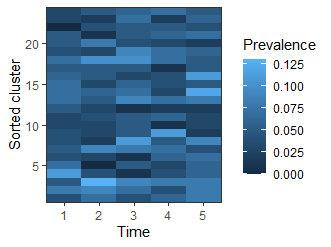
\includegraphics[width=7.1cm]{data1.png}
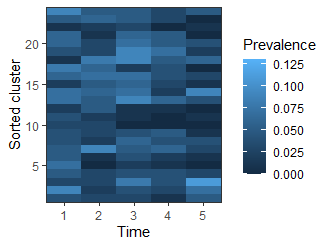
\includegraphics[width=7.1cm]{data05.png}
\caption{Cluster-level data simulated for $\text{RR}=1$ (left) and $\text{RR}=0.5$ (right). The clusters are sorted such that clusters $1$--$6$ cross over at time 2, clusters $7$--$12$ cross over at time 3, and so on. The prevalence at each cluster-time is computed from 100 individual-level units.}
\label{fig:data}
\end{figure}

For comparison, Figure~\ref{fig:data1000} shows the same plots but with the prevalence computed over 1000 units at each cluster-time. The stepped wedge pattern is now clearly visible when $\text{RR}=0.5$.

\begin{figure}[H]
\centering
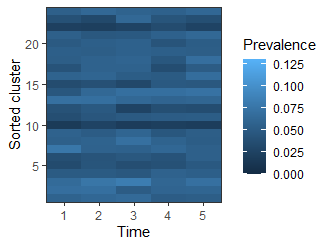
\includegraphics[width=7.1cm]{data1_1000.png}
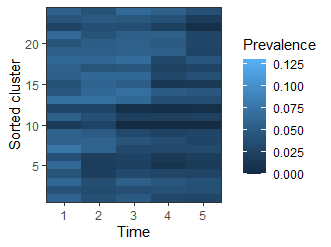
\includegraphics[width=7.1cm]{data05_1000.png}
\caption{Cluster-level data simulated for $\text{RR}=1$ (left) and $\text{RR}=0.5$ (right). The clusters are sorted such that clusters $1$--$6$ cross over at time 2, clusters $7$--$12$ cross over at time 3, and so on. The prevalence at each cluster-time is computed from 1000 individual-level units.}
\label{fig:data1000}
\end{figure}

\end{document}